\documentclass[a4paper, 10pt]{article}

%\usepackage{scalefnt}
%\usepackage{parcolumns}

\usepackage{newclude}
% Zum Einbinden in die Zusammenfassungs-files

\usepackage{amsmath,amsthm,amsfonts,amssymb} % Verbesserter Mathesatz
\usepackage{algorithm2e}
\usepackage{bigfoot} % komplexe Fußnotenapparate(Fußnoten in Fußnoten und andere Späße)%
\usepackage{colortbl}
\usepackage[T1]{fontenc} % normaler erweitere Zeichnesatz
\usepackage{framed, color}  % Ramenpaket für zum Einfügen von schönen Ramen
\usepackage{graphicx}
\usepackage{hyperref} %used for link to creative commons license
\usepackage{listings} %for code-listings (inkl. Tab-Styling)
\usepackage{marvosym}
\usepackage{marginnote}
\usepackage{microtype} % div. Verbesserungen des Schriftsatzes (Grauwert, opt. Randausgleich, Zeilenumbruch)
%\usepackage{multirow}
\usepackage{multicol} %use this with next line for vertical divided environment
%\setlength\columnseprule{.4pt}:465
\usepackage[ngerman]{babel} % Neue Rechtschreibung
\usepackage{pifont}
\usepackage[sans]{dsfont} %für alternative Mengensymbole
\usepackage{stmaryrd} %u.a. für \lightning
\usepackage{tikz} % für Diagramme(Dia!) und Bilder (z.B. *.eps)/für ER-Diagramme/für UML-Diagramme
%\usepackage{tikz-er2} %  er-diagramme
\usepackage{tikz-uml} % uml-Diagramme
\usepackage{units} % z.B. fuer \nicefrac{}{}
\usepackage[utf8]{inputenc} % utf8 für den Editor
\usepackage{wasysym} %u.a. für \lightning
\usepackage{xcolor}


\usetikzlibrary{shapes,decorations,arrows,fit,backgrounds} %Zum diversen zeichen%
%\usetikzlibrary{automata} % für den CFlipper, wenn es den soweit ist			%
\usetikzlibrary{positioning} % positionierung
%\usetikzlibrary{shadows} % fuer schoene schlagschatten
\usetikzlibrary{automata} % für Automaten

%%%%%%%%%%%%%%%%%%%%%%%%%%%
%  Formatierung der Seite
%%%%%%%%%%%%%%%%%%%%%%%%%%%
\usepackage{fancyhdr}
\pagestyle{fancy}		% für den footer										%
\renewcommand{\headrulewidth}{0pt} % damit oben kein dummer Strich kommt		%
\fancyhead{}
\topmargin -2cm 		% Oberer Rand											%
\textheight 25cm		% Texthöhe												%
\textwidth 16.0 cm		% Textbreite											%
\oddsidemargin -0.1cm 	% Warum?												%
\newcommand{\Gruppe}[2]
{
	\lfoot{#1}
	\rfoot{#2}
}
\colorlet{shadecolor}{gray!25} % Farbe für graue Box definieren
%%%%%%%%%%%%%%%%%%%%%%%%%%%%%%%%%%%%%%%%%%%%%%%%%%%%%%%%%%%%%%%%%%%%%%%%%%%%%%%%%
%Farben die definiert werden zum schreiben und zeichnen							%
%%%%%%%%%%%%%%%%%%%%%%%%%%%%%%%%%%%%%%%%%%%%%%%%%%%%%%%%%%%%%%%%%%%%%%%%%%%%%%%%%
\xdefinecolor{schwarz}{HTML}{000000}
\xdefinecolor{dunkelGruen}{HTML}{007D00}
\xdefinecolor{dunkelBlau}{HTML}{0000A0}
\xdefinecolor{dunkelRot}{HTML}{A00000}
\xdefinecolor{dunkelGelb}{HTML}{FFAA00}
\xdefinecolor{hellesGelb}{HTML}{FFCC00}
\colorlet{dGreen}{dunkelGruen}
\colorlet{dBlue}{dunkelBlau}
\colorlet{dRed}{dunkelRot}
\colorlet{dYellow}{dunkelGelb}

%%%%%%%%%%%%%%%%%%%%%%%%%%%%%%%%%%%%%%%%%%%%%%%%%%
%Farbliche Ausgaben:
%Parameter #1: Text oder Mathematische formel...
%z.B. : \gruen{Hallo Welt Test!}
%%%%%%%%%%%%%%%%%%%%%%%%%%%%%%%%%%%%%%%%%%%%%%%%%%

\newcommand{\yellow}[1]{\textcolor{dYellow}{#1}}
\newcommand{\gray}[1]{\textcolor{gray}{#1}}
\newcommand{\red}[1]{\textcolor{red}{#1}}
\newcommand{\green}[1]{\textcolor{green}{#1}}
\newcommand{\blue}[1]{\textcolor{blue}{#1}}
\newcommand{\dGreen}[1]{\textcolor{dGreen}{#1}}
\newcommand{\dBlue}[1]{\textcolor{dBlue}{#1}}
\newcommand{\dRed}[1]{\textcolor{dRed}{#1}}

%%%%%%%%%%%%%%%%%%%%%%%%%%%%%%%%%%%%%%%%%%%%%%%%
%Konfiguration für das darstellen von Quelltext
%%%%%%%%%%%%%%%%%%%%%%%%%%%%%%%%%%%%%%%%%%%%%%%%
\lstset
{
	language=Java, % oder C++, Pascal, {[77]Fortran}, ...
	numbers=left, % Position der Zeilennummerierung
	firstnumber=auto, % Erste Zeilennummer
	basicstyle=\ttfamily, % Textgröße des Standardtexts
	keywordstyle=\ttfamily\color{dRot}, % Formattierung Schlüsselwörter
	commentstyle=\ttfamily\color{dGruen}, % Formattierung Kommentar
	stringstyle=\ttfamily\color{dBlau}, % Formattierung Strings
	numberstyle=\tiny, % Textgröße der Zeilennummern
	stepnumber=1, % Angezeigte Zeilennummern
	numbersep=5pt, % Abstand zw. Zeilennummern und Code
	aboveskip=15pt, % Abstand oberhalb des Codes
	belowskip=11pt, % Abstand unterhalb des Codes
	captionpos=b, % Position der Überschrift
	xleftmargin=10pt, % Linke Einrückung
	frame=single, % Rahmentyp
	breaklines=true, % Umbruch langer Zeilen
	showstringspaces=false, % Spezielles Zeichen für Leerzeichen
	tabsize=2,
	texcl=true
}

%%%%%%%%
% Kopf
%%%%%%%%
\newcommand{\Header}[3]
{
	{\footnotesize \parindent0em
		{\sc Universität Konstanz}                \hfill #1 \\
		{\sc Fachbereich Informatik \& Informationswissenschaft} \hfill #2 \\
		#3 \hfill \today
	}
}

%%%%%%%%%%%%%%%%%%%%%%%
% load some java code
% \loadJava{file}
%%%%%%%%%%%%%%%%%%%%%%%
\newcommand{\loadJava}[1]
{
	\lstinputlisting[language=Java]{#1.java}
}

%%%%%%%%%%%%%%%%%%%%%%%
% load some cpp code
% \loadCpp{file.cpp}
%%%%%%%%%%%%%%%%%%%%%%%
\newcommand{\loadCpp}[1]
{
	\lstinputlisting[language=C++]{#1}
}

%%%%%%%%%%%%%%%%%%%%%%%%%%%%%
% load some code
% \loadCode{Python}{file.py}
%%%%%%%%%%%%%%%%%%%%%%%%%%%%%
\newcommand{\loadCode}[2]
{
	\lstinputlisting[language=#1]{#2}
}

%%%%%%%%%%%%%%%%%%%%%%%%%%%%%%%%%%%%%%%%%%%%%%%%%%%%%%%%%%%%%%%%%%%%%%%
% some symbols
%%%%%%%%%%%%%%%%%%%%%%%%%%%%%%%%%%%%%%%%%%%%%%%%%%%%%%%%%%%%%%%%%%%%%%%
\newcommand{\correct}{\green{\text{\ding{52}}}} %for use in text and math
\newcommand{\wrong}{\red{\text{\ding{56}}}} %for use in text
\newcommand{\tflash}{$\yellow{\lightning}$} %for use in text
\newcommand{\mflash}{\yellow{\lightning}} %for use in math
\newcommand{\follows}{$\Rightarrow$} %used so often...
\newcommand{\good}{\item[\dGreen{\ding{58}}]} %an item with a green plus as bullet point
\newcommand{\bad}{\item[\red{\Emailct}]} %better icon for bad items
\newcommand{\note}[1]{\red{\marginnote{#1}}} %add a red margin note
\newcommand{\fitem}{\item[\follows]} %items with a follows arrow
\newcommand{\hm}{\ensuremath{\overset{-\mkern-11mu-\mkern-3.5mu\rhook}{\smash{\odot}\rule{0ex}{.46ex}}\underline{\hspace{0.5em}}\overset{-\mkern-11mu-\mkern-3.5mu\rhook}{\smash{\odot}\rule{0ex}{.46ex}}}}

%%%%%% make emph bold instead of italic %%%%%
\makeatletter
\DeclareRobustCommand{\em}{%
  \@nomath\em \if b\expandafter\@car\f@series\@nil
  \normalfont \else \bfseries \fi}
\makeatother

%%%%%%%%%%%%%%%%%%%%%%%%%%%%%%%%%%%%%%
% languages for \loadCode
%ABAP		IDL				Plasm
%ACSL		inform			POV
%Ada		Java			Prolog
%Algol		JVMIS			Promela
%Ant		ksh				Python
%Assembler	Lisp			R
%Awk		Logo			Reduce
%bash		make			Rexx
%Basic		Mathematica1	RSL
%C			Matlab			Ruby
%C++		Mercury			S
%Caml		MetaPost		SAS
%Clean		Miranda			Scilab
%Cobol		Mizar			sh
%Comal		ML				SHELXL
%csh		Modula-2		Simula
%Delphi		MuPAD			SQL
%Eiffel		NASTRAN			tcl
%Elan		Oberon-2		TeX
%erlang		OCL				VBScript
%Euphoria	Octave			Verilog
%Fortran	Oz				VHDL
%GCL		Pascal			VRML
%Gnuplot	Perl			XML
%Haskell	PHP				XSLT
%HTML		PL/I
%%%%%%%%%%%%%%%%%%%%%%%%%%%%%%%%%%%%%%

\begin{document}

\Gruppe{Stephan Heidinger}{fses 10}
\Header{Functional Safety in Embedded Systems}{Session 10 - Formal Methods for Functional Safety II}

\section*{Formal Methods for Safety Assessment (ctd)}
\subsubsection*{Model Checking}
\begin{itemize}
    \item complement simulation and testing
    \item system is modeled as state transition system
    \item check automatically, that specifications are met (exhaustively explore state space)
    \item finite models \follows guaranteed termination
    \item counterexample is produced, when failure state is found
    \item check a \emph{Kripke}-structure \follows may be exponential in number of components
    \item \emph{explicit model checking} SPIN: explicitly compute states
    \item \emph{symbolic model checking} SMV, NuSMV, VIS\follows manipulate sets of states and transitions
    \item \emph{binary decision diagrams} SMV: representation for logic formulae
    \item \emph{bounded model checking} (symbolic) bound steps to a value $k$, uses modern SAT solvers
    \item often run bdd and bmc in parallel, the first one to finishes, wins
    \item \emph{timed model checking} UPAAL, KRONOS
    \item \emph{probabilistic model checking} PRISM, MRMC
    \item \emph{partial order reduction} \follows reduce state space
    \item \emph{symmetry reduction} exploit symmetry in model
\end{itemize}

\subsubsection*{Using Model Checking for Requirements Validation}
\begin{itemize}
    \item validate a set of requirements (assumes, that requirements meet end-user expectations)
    \item RAT tool provides way to asses quality of requirements
    \begin{itemize}
        \item \emph{property simulation} \follows behavior associated with each requirement
        \item \emph{property assurance} check for logical consistency (=freedom from contradictions)
        \begin{itemize}
            \item if requirements are logically inconsistent \follows find subset, that is explanation for inconsistency
        \end{itemize}
    \end{itemize}
\end{itemize}

\subsubsection*{Using Model Checking for Property Verification}
\begin{itemize}
    \item build formal model for system (state transition system)
    \item checked by model checker
    \item FSAP tool for formal verification and safety analysis, GUI on top of NuSMV
\end{itemize}

\subsection*{Formal Safety Analysis}
\begin{itemize}
    \item ESACS and ISAAC \follows ESACS methodology supported by formal methods, to assist system development and safety analysis
    \item shared formal notations between design and safety analysis
    \item decoupling between nominal model and fault model
    \begin{enumerate}
        \item formal model (design or safety engineer) \follows \emph{nominal system model} (only nominal behavior)
        \item \emph{fault injection}: put nominal model into failure modes \follows extended model through model extension
    \end{enumerate}
    \begin{center}
        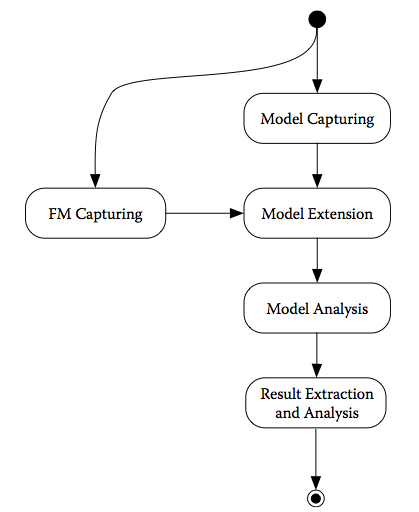
\includegraphics[width=.5\linewidth]{images/esacs.png}
    \end{center}
\end{itemize}

\subsubsection*{Fault Injection}
\begin{center}
    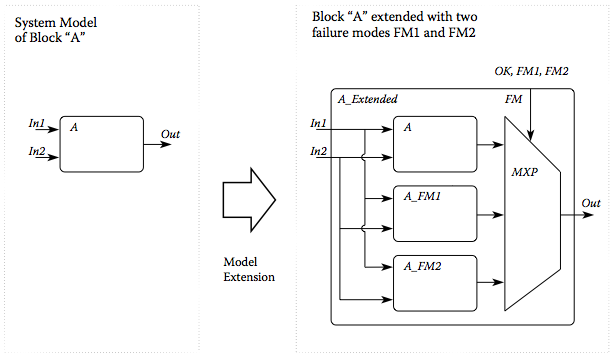
\includegraphics[width=\linewidth]{images/faultinjection.png}
\end{center}

\subsubsection*{Fault Models and Model Extension}
\begin{itemize}
    \item FSAP generic failure mode library: library of typical failure modes to be injected
    \item model extension takes specification of fault to be added
    \item \emph{fault configuration} subset of failure mode variables
\end{itemize}

\subsubsection*{Fault Tree Generation}
\begin{itemize}
    \item fault tree can be represented as collection: of minimal cut sets TLE and and conjunction of corresponding basic faults
    \item generation of fault tree:
    \begin{itemize}
        \item need to remember, if fault has been activated during iterative traversal
        \begin{center}
            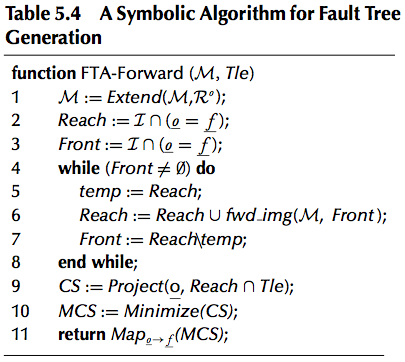
\includegraphics[width=.5\linewidth]{images/faultTreeGeneration.png}
        \end{center}
    \end{itemize}
\end{itemize}

\subsubsection*{FMEA Table Generation}
\begin{itemize}
    \item input: set of failure modes + set of events to be analyzed
    \item FSAP does this somehow (magic?)
\end{itemize}

\subsection*{Industrial Application of Formal Methods}
\subsubsection*{IBMs Customer Information Control System}
\begin{itemize}
    \item more than $750\;000$ lines of code
    \item more than $2\;000$ pages of formal specifications produced
    \item reduction in development cost of about $9\%$
\end{itemize}

\subsection*{Conclusion}
\begin{itemize}
    \item formal methods in design and development become more pervasive
    \item CounterExample Guided Abstraction Refinement (CEGAR) builds set of abstraction from set of predicates
    \item nontrivial: systems with both digital and analogue parts (\emph{hybrid systems})
\end{itemize}

\end{document}
